\documentclass[a4paper]{article}
\usepackage{amsmath}
\usepackage{hyperref}
\usepackage{cleveref}
\usepackage[italian]{babel}
\usepackage{graphicx}
\usepackage[margin=2cm]{geometry}
\usepackage{subcaption}
\DeclareMathOperator*{\sca}{\textrm{sca}}
\title{Progetto Controlli Automatici T \\ 1C - Controllo del posizionamento di un link flessibile}
\author{Riccardo Corradini \and Luigi di Nuzzo \and Kevin Michael Frick \and Davide Ragazzini \and Antony Zappacosta}
\begin{document}
\maketitle
\section{Descrizione e requisiti del sistema}
Nella nuova applicazione della azienda che commissiona il progetto si prevede di utilizzare una struttura meccanica particolarmente leggera. 
Questa però presenta il problema di una flessibilità non trascurabile intrinseca nei componenti meccanici utilizzati. 
Ciò rende difficile il posizionamento dell’estremità non attuata in una posizione fissa desiderata.
L’intera struttura in questione è modellizzata da \cref{eqn:model} ed è schematizzata come in \cref{fig:sys_schem}.
\begin{equation}
    \label{eqn:model}
    \begin{array}{lclcc}    
    \dot{x_1} & = & f_1 (x_1, x_2, x_3, x_4) & = & x_2 \\
    \dot{x_2} & = & f_2 (x_1, x_2, x_3, x_4) & = & \frac{-M g L \sin (x_1) - K (x_1 - x_3) - \rho (x_2 - x_4)}{J} \\
    \dot{x_3} & = & f_3 (x_1, x_2, x_3, x_4) & = & x_4 \\
    \dot{x_4} & = & f_4 (x_1, x_2, x_3, x_4) + g(u) & = & \frac{K(x_1 - x_2) + \rho (x_2 - x_4) + u}{I}\\
    y & = & f_y (x_1, x_2, x_3, x_4) & = & x_1
    \end{array}
\end{equation}
\begin{figure}[h]
    \centering
 \begin{subfigure}{0.45\textwidth}
    \centering
    \includegraphics[width=\textwidth]{schematic.png}
    \caption{Schema del modello fisico del sistema.}
    \label{fig:sys_schem}
 \end{subfigure}
 ~
 \begin{subfigure}{0.45\textwidth}
    \centering
    \includegraphics[width=\textwidth]{control_sys.png}
    \caption{Schema di controllo del sistema linearizzato.}
    \label{fig:sys_cont}
 \end{subfigure}
\end{figure}
La variabile $\theta$ in \cref{fig:sys_schem} viene descritta dallo stato $x_1$ e rappresenta l’angolo rispetto ad un piano di riferimento fisso che la massa concentrata del link traccia nel suo moto. $\theta_m$ (nelle equazioni $x_3$) rappresenta l’angolo di rotazione del motore, il cui input $u$ al sistema è la coppia applicata $\tau_m$. $K, \rho, L, Mp, Jp, I$ sono rispettivamente: la costante elastica del link, il suo coefficiente di attrito dinamico, la lunghezza, la massa concentrata sull’estremità non attuata, il momento d’inerzia della stessa massa e il momento d’inerzia del link equivalente visto dal punto di vista del motore.
Ai fini dello sviluppo del controllo dell’impianto si vuole ottenere la struttura in \cref{fig:sys_cont}.

Come prima analisi il sistema non lineare deve essere considerato nell’intorno di un punto di equilibrio, i cui valori $(\bar{x}, \bar{u})$ sono definiti nella tabella, e linearizzato nello stesso intorno.
Il modello nella \cref{eqn:model} è stato quindi linearizzato nell’intorno di $(\bar{x}, \bar{u})$ servendosi della \cref{eqn:linearization_calc} ottenendo la \cref{eqn:linearization}.

\begin{equation}
    \label{eqn:linearization_calc}
    \begin{array}{rcl}   
        \nabla f_1 & = &(0, 1, 0, 0) \\
        \nabla f_2 & = &\frac{1}{J_p} (-M_p g L \cos(x_1) - K, - \rho, K, \rho) \\
        \nabla f_3 & = & (0, 0, 0, 1)\\
        \nabla f_4 & = & \frac{1}{I} (K, \rho, -K, -\rho) \\
        \nabla f_y & = & (1, 0, 0, 0)  \\
        \frac{dg}{du} & = & \frac{u}{I}
    \end{array}
\end{equation}

\begin{equation}
    \label{eqn:linearization}
A = \begin{pmatrix}0 & 1 & 0 & 0 \\
    -\frac{K}{J} & -\frac {\rho}{J} & \frac{K}{J} & \frac{\rho}{J} \\
    0    &   0    &   0    &   1\\
    \frac{K}{I} & \frac{\rho}{I} & -\frac{K}{I} & \frac{\rho}{I}
\end{pmatrix};
B = (0, 0, 0, \frac{1}{I})^T;
C = (1, 0, 0, 0);
D = (0);
\end{equation}

È necessario poi passare dalla rappresentazione nello spazio degli stati al dominio di Laplace utilizzando la trasformata di Laplace, ottenendo la funzione di trasferimento nella \cref{eqn:G}.

\begin{equation}
    \label{eqn:G}
    G(s) = \frac{1000 (s+15)}{s^2 (s^2 + 30s + 450)}
\end{equation}

Per l’applicazione che l’azienda ha in mente si devono rispettare per il sistema linearizzato determinate caratteristiche:
\begin{enumerate}
    \item Errore a regime nullo con riferimento a gradino con ampiezza $w(t) = W \sca(t)$.
    \item Per garantire una certa robustezza del sistema si deve avere un margine di fase $\phi_m \geq 45^\circ$.
    \item Il sistema può accettare una sovraelongazione percentuale al massimo dell’1\% : $S\% \leq 1\%$.
    \item Tempo di assestamento all'1\% $T_{a1} = 0.8$ (opzionalmente 0.4).
    \item Abbattimento del rumore di 20 volte.
\end{enumerate}

Il rumore si fa sentire a $\omega_n > 200 rad/s$ con ampiezza $A_n = 0.05$.
    
Dopo aver definito i parametri del sistema, calcolato le matrici linearizzate e la funzione di trasferimento, si definisce su MATLAB l’intervallo di frequenze che sarà mostrato nel diagramma di Bode: $\omega \in [10^{-2}, 10^5]$.

\begin{figure}[h]
    \centering
    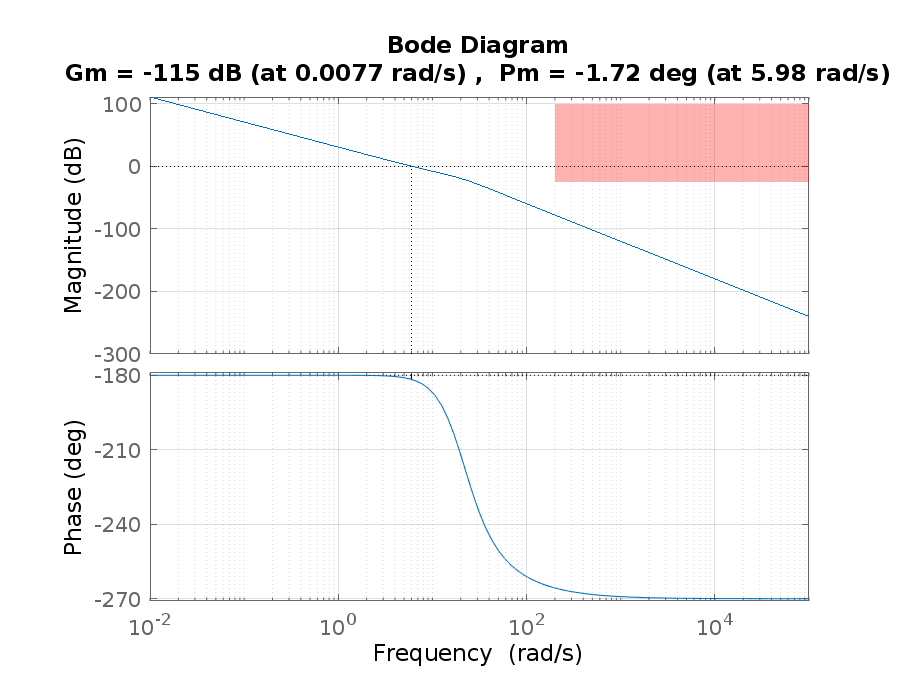
\includegraphics[width=0.6\textwidth]{bode_G}
    \caption{Diagramma di Bode del sistema in anello aperto}
    \label{fig:bode_G}
\end{figure}

\section{Requisiti sul margine di fase}
Il requisito sulla sovraelongazione si traduce in un requisito sul margine di fase che è maggiore di quello specificato.
Tuttavia, durante la sintesi del controllore si è notato che anche non rispettando questo requisito è possibile avere un sistema che rispetti le specifiche di sovraelongazione e abbia un tempo di assestamento ottimale.

\begin{equation}
    \xi = \sqrt{\frac{\log(S_{max})^2}{(\pi^2+\log(S_{max})^2)}} \approx 0.826
    \label{eqn:xi}
\end{equation}

\begin{equation}
    \phi_m \approx \xi \cdot 100 \approx 83^\circ
    \label{eqn:phim}
\end{equation}

\section{Definizione del regolatore}
Per avere errore a regime nullo è necessario che $L(s)$ abbia un polo nell'origine, ma $G(s)$ ne ha due, che abbassano di molto la fase: si progetta quindi $R(s)$ in modo che abbia uno zero vicino all'origine che cancelli il polo.

Ci si serve di due reti anticipatrici, una con punto medio in $\omega_1 = 1/ (T_1 \sqrt{\alpha_1}) \approx 5 \cdot 10^{-1}$ e un'altra con punto medio in $\omega_2 = 1/ (T_2 \sqrt{\alpha_2}) \approx 7 \cdot 10^{-3}$;
La prima rete anticipatrice ha una larghezza di banda di circa una  decade, uno zero a $\omega_{z1} \approx -0.06$ e un polo a $\omega_{p1} \approx -70$. 
La seconda rete anticipatrice ha una larghezza di banda di circa tre decadi, uno zero a $\omega_{z2} \approx -20$ e un polo a $\omega_{p2} \approx -10^{-3}$.

I parametri delle reti anticipatrici sono $T_1 = 17.42, \alpha_1 = 8.2 \cdot 10^{-4}, T_2 = 0.05, \alpha_2 = 0.02$.

Il guadagno statico del regolatore è $\mu_s = 3.4 \cdot 10^{-2}$.

La funzione di trasferimento del regolatore è data dalla \cref{eqn:R}.
\begin{equation}
    \label{eqn:R}
    R(s) = \frac{2073.2 (s+20) (s+0.05741)}{(s+1000) (s+70.01)}
\end{equation}
\begin{figure}[h]
    \centering
    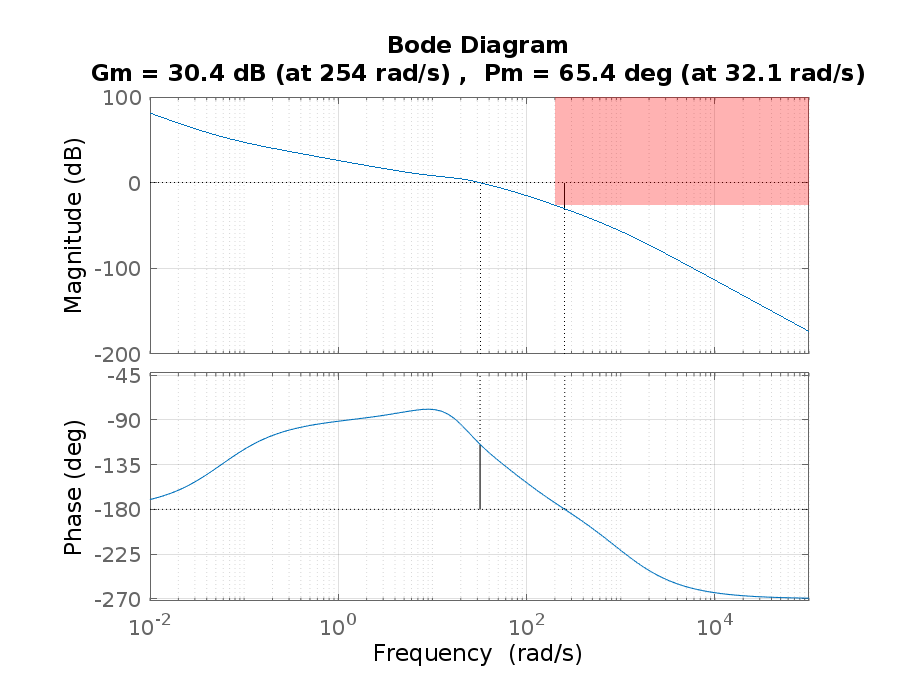
\includegraphics[width=0.6\textwidth]{bode_L}
    \caption{Diagramma di Bode del sistema con regolatore.}
    \label{fig:bode_L}
\end{figure}
\section{Risposta del sistema in anello chiuso con regolatore}
Il sistema linearizzato non ha sovraelongazione e ha un tempo di assestamento all'1\% pari a 0.3817 secondi (misurato con la funzione MATLAB \texttt{stepinfo}).
\begin{figure}[h]
    \centering
    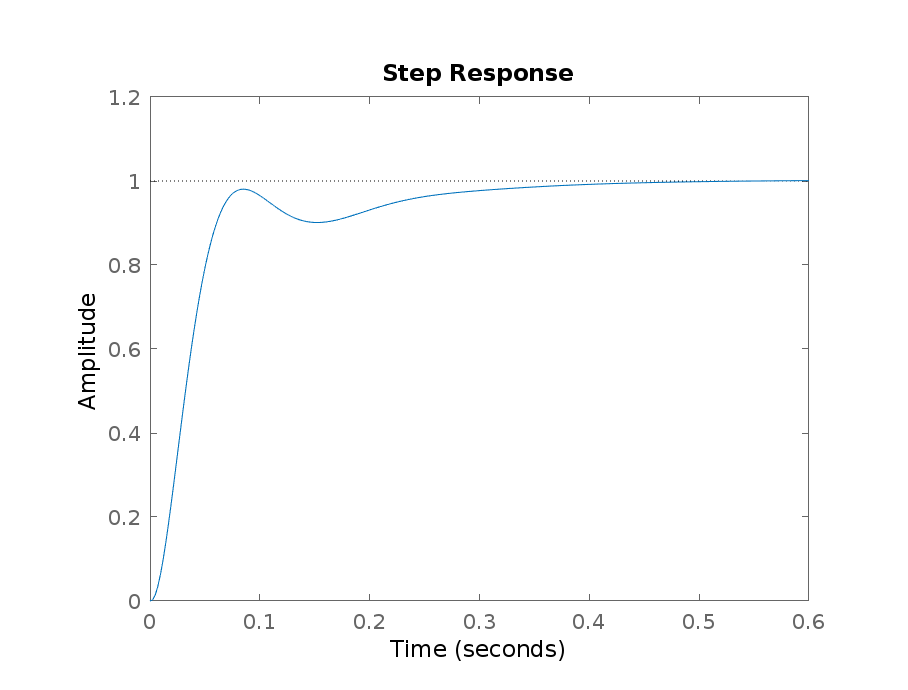
\includegraphics[width=0.5\textwidth]{step}
    \caption{Risposta allo scalino del sistema in anello chiuso con regolatore}
    \label{fig:step}
\end{figure}

\section{Simulink}
Il sistema è stato simulato, sia nella sua versione linearizzata che in quella non linearizzata, servendosi del pacchetto software Simulink. 
\begin{figure}[h]
    \centering
    \includegraphics[width=0.7\textwidth]{Simul1C.pdf}
    \caption{Sistema linearizzato.}
    \label{fig:sim_lin}
\end{figure}
\begin{figure}[h]
    \centering
    \includegraphics[width=0.7\textwidth]{NonLin1C.pdf}
    \caption{Sistema non linearizzato.}
    \label{fig:sim_nonlin}
\end{figure}
La risposta allo scalino del sistema linearizzato ricalca quella ottenuta con la funzione \texttt{step} di MATLAB.
La risposta allo scalino del sistema non linearizzato mostra che è possibile ottenere stabilità solamente con valori di ingresso a scalino inferiori a $w = \frac{W}{8} \sca(t)$. 
\begin{figure}[h]
    \centering
\begin{subfigure}[t]{0.3\textwidth}
    \centering
    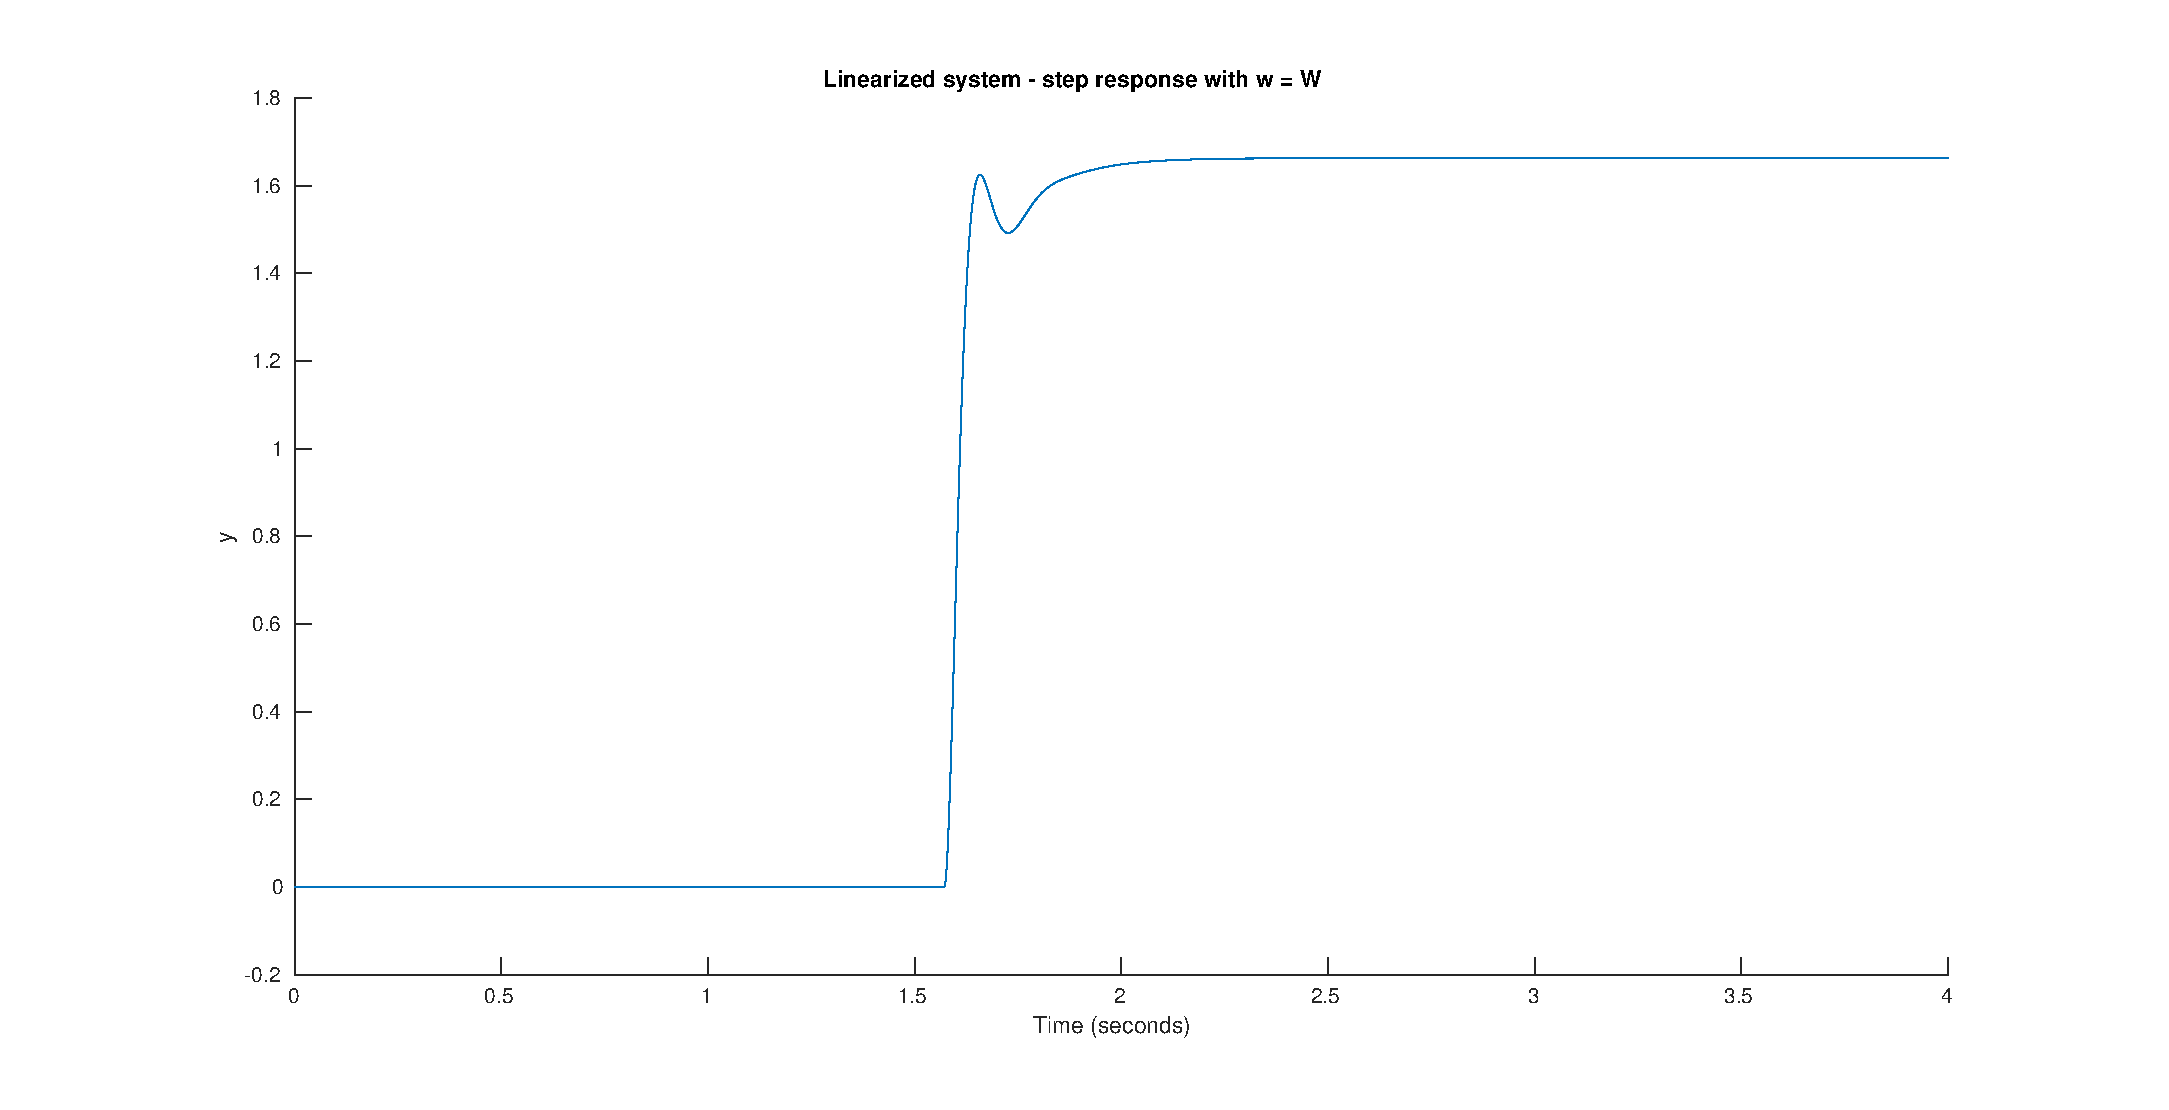
\includegraphics[width=\textwidth]{step_lin}
    \caption{Risposta allo scalino del sistema linearizzato}
    \label{fig:step_sim_lin}
\end{subfigure}
~
\begin{subfigure}[t]{0.3\textwidth}
    \centering
    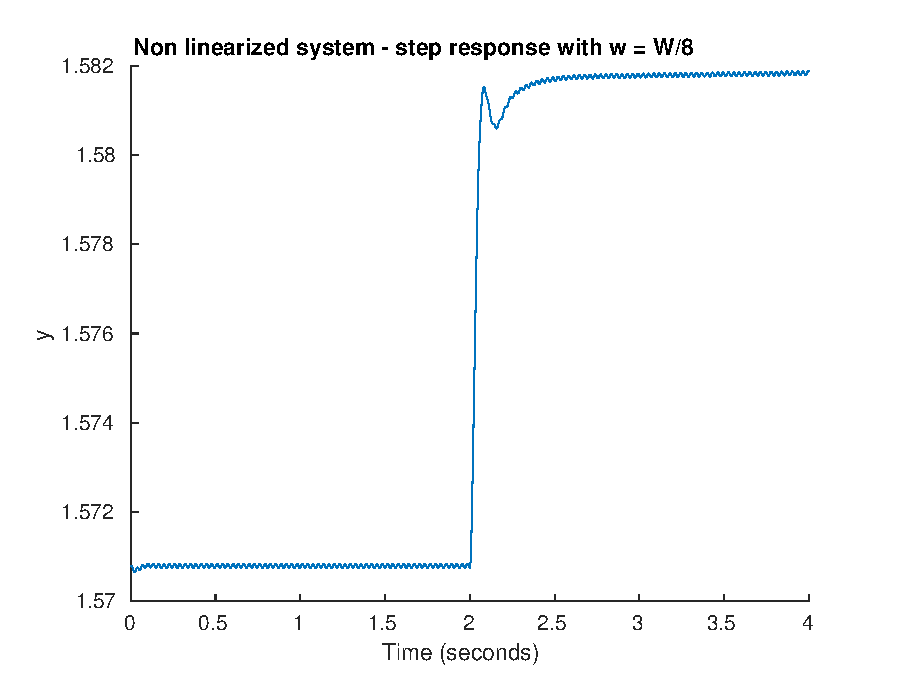
\includegraphics[width=\textwidth]{step_nonlin_short}
    \caption{Risposta allo scalino del sistema non linearizzato}
    \label{fig:step_sim_nonlin}
\end{subfigure}
~
\begin{subfigure}[t]{0.3\textwidth}
    \centering
    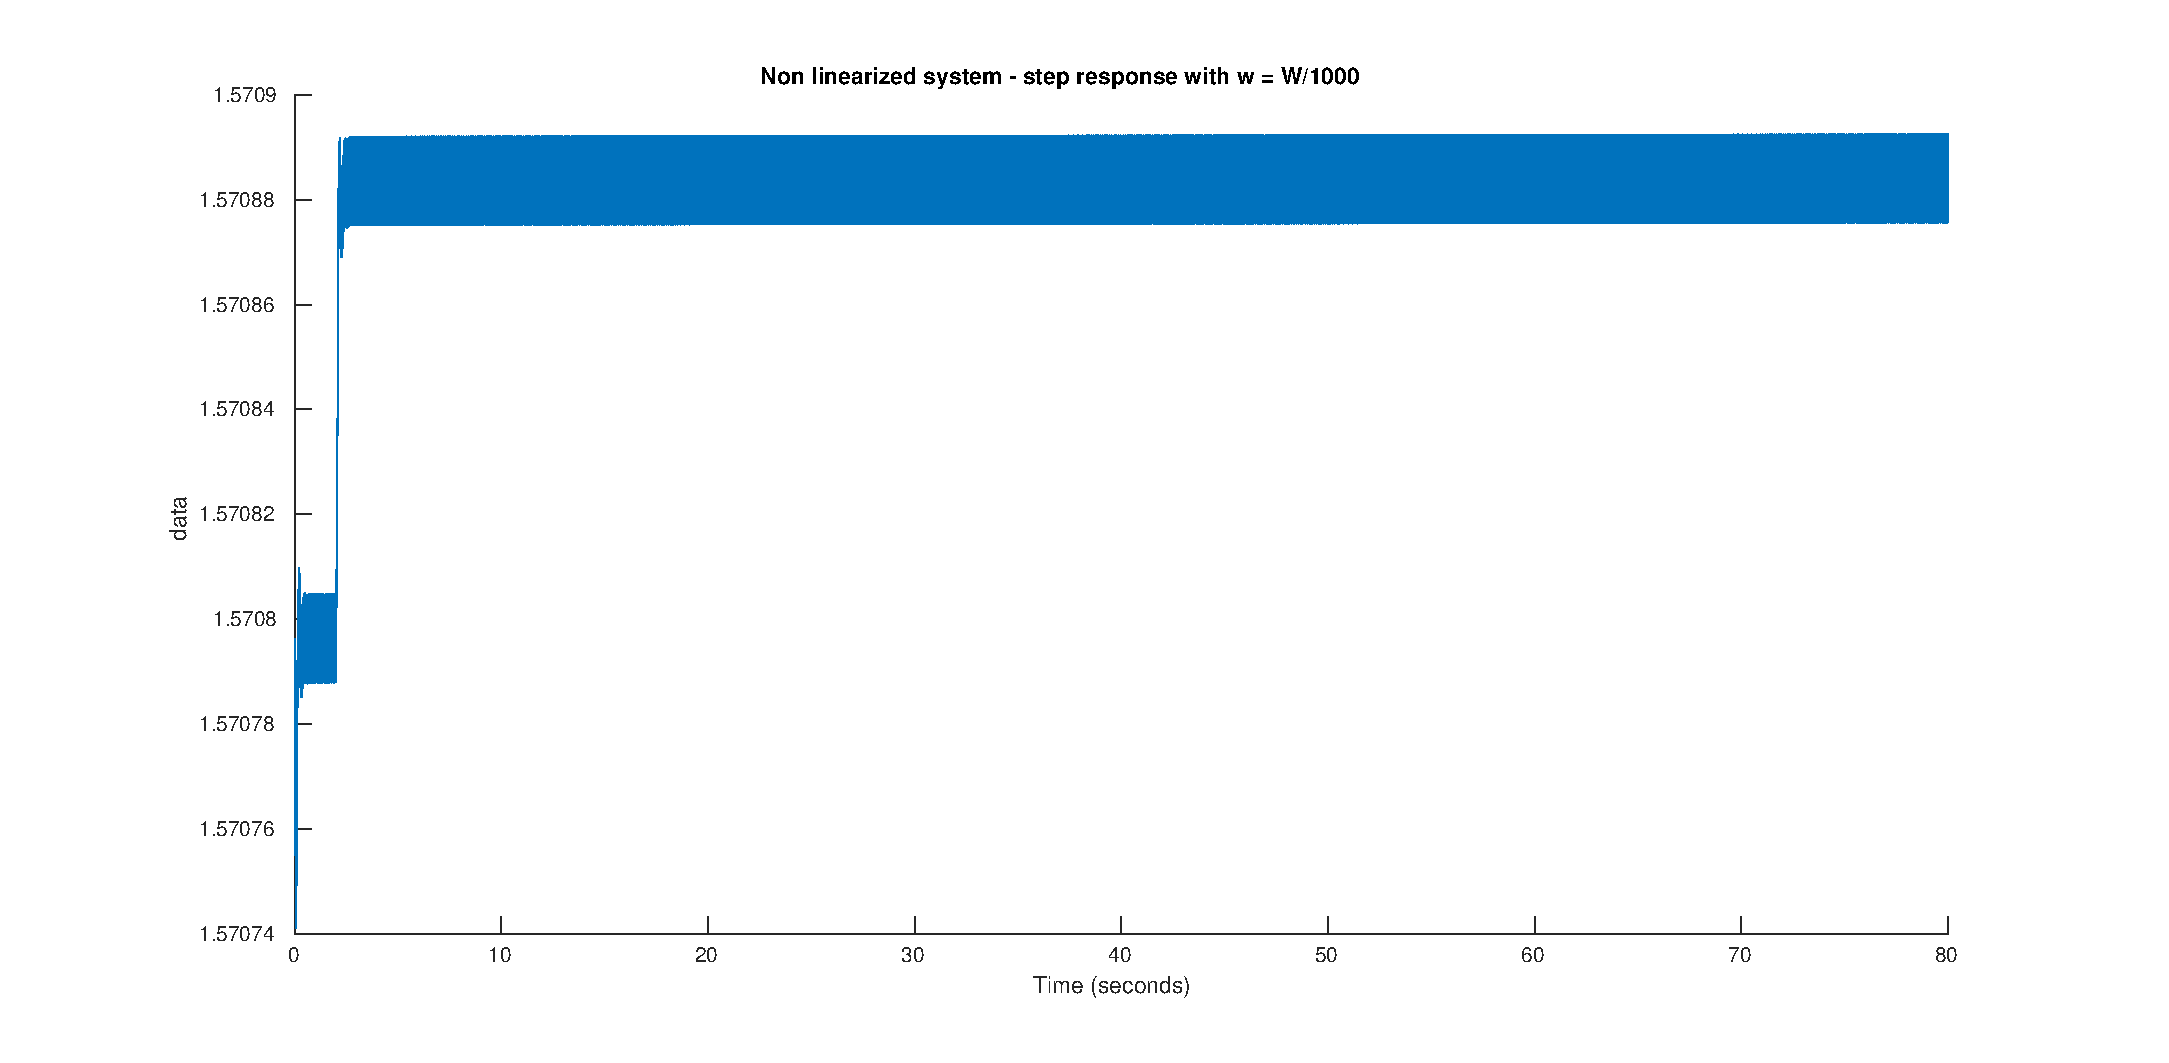
\includegraphics[width=\textwidth]{step_nonlin_long}
    \caption{Risposta allo scalino del sistema non linearizzato che mostra la lunga coda di assestamento.}
    \label{fig:step_sim_nonlin_long}
\end{subfigure}
\end{figure}
\end{document}